\documentclass[11pt,a4paper]{ctexart}
\usepackage[margin=2.35cm]{geometry}
\usepackage{amsmath,amssymb,bm}
\usepackage{booktabs}
\usepackage{graphicx}
\usepackage{xcolor}
\usepackage{caption}
\usepackage[colorlinks=true,linkcolor=blue!50!black,urlcolor=blue!50!black]{hyperref}
\setCJKmainfont{Noto Sans CJK SC}
\setCJKsansfont{Noto Sans CJK SC}
\captionsetup{font=small}
\renewcommand{\arraystretch}{1.15}

\title{\bfseries 双 MCT 猫道扭转偏差的理论推导修复\\
\large 双索组滚转升级、双簇端口凝聚与"审计部件扭转可达域"的定量结论}
\author{双 MCT 猫道简化模型复算（Fable 理论推导稿）}
\date{2026 年 8 月 27 日}

\begin{document}
\maketitle

\noindent\fbox{\parbox{\dimexpr\linewidth-2\fboxsep}{\textbf{性质声明（not\_a\_scientific\_claim）}：本文为理论推导与复算记录。全部输入参数取自仓库既有审计数据（哈希与出处见附录），无任何拟合或对标调参；不宣布"复现附件"或任何科学成功。附件 2--3 表 4--1 的参考频率仅作对照，不参与任何模型构建环节。}}

\section{任务、结论与阅读地图}

\textbf{任务}：附件 2--3 表 4--1 与双 MCT 模型正式配对后，扭转族（T）偏差为
$-28.22\%/-11.96\%/-8.46\%$（TA1/TS1/TS2），此前已定位为"平面化等效丢失幅内扭转"。
本文通过理论推导重建等效层级，试图修复该缺陷，并给出推导全过程。

\textbf{完成的修复（结构层面）}：
\begin{enumerate}
  \item \textbf{双索组等效}：每幅承重索束按实索排布拆为 $\pm b_B$ 两个等效索组
        （$b_B=1.858$ m，16 根 $\phi50$ 偏距的均方根），门架索束拆为 $\pm b_T$
        （$b_T=1.962$ m，6 根 $\phi54$）。共模动力学严格不变，幅内滚转的几何刚度
        $\sum T_i y_i^2$ 与惯量 $\sum m_i y_i^2$ 按实索排布精确恢复（第 \ref{sec:twoline} 节）。
  \item \textbf{双簇端口凝聚}：普通门架与横通道站改用"每接口两个索簇平动子端口"的
        凝聚矩阵（转角全部自由凝聚）。矩阵恰有 6 个刚体零模态、无多余机构，
        滚转成为客观可观量，横梁在簇间的柔性得到保留（第 \ref{sec:cluster} 节）。
  \item \textbf{二期质量空间化}：963.811 t 二期集中质量按质量空间化审计 V2.0 的
        33003 个真实坐标分配，滚转惯量客观化；总质量闭合误差 $9.7\times10^{-10}$ t
        （第 \ref{sec:mass} 节）。
  \item 附带治愈两类非物理分支：双索组"呼吸"机构与 M37 起的门架索横向解耦分支
        均被簇端口客观约束（第 \ref{sec:results} 节）。
\end{enumerate}

\textbf{核心理论结论（扭转可达域）}：在上述全审计装配下，表 4--1 的 T 族误差几乎不变
（$-28.62\%/-11.83\%/-9.03\%$）。这不是实现失败，而是可以从两条引理严格解释的结构事实：
\begin{itemize}
  \item \textbf{系统扭转钉扎}：双幅整体扭转的频率被"摆式物理"钉在竖弯族上
        （张力与质量的横向二阶矩同构），模型实测 TA1 与 VA1 分裂仅 $0.069\%$；
  \item \textbf{幅内滚转锁定}：审计钢结构（门架框架 $4.7\times10^{6}$、横通道
        $1.0\text{--}2.6\times10^{8}$ N·m/rad）把幅内滚转分支推到 $1.0$ Hz 以上，
        比附件 TA1 高一个量级。
\end{itemize}
因此\textbf{任何由现有审计部件客观装配的模型，在 0.08--0.17 Hz 都不可能出现独立扭转分支}；
由附件 TA1 反推，附件模型隐含的每品门架有效滚转约束约为 $1.5\times10^{4}$ N·m/rad，
比审计刚接值低 2--4 个数量级。
\textbf{2026-08-27 补充（第 \ref{sec:drawings} 节）}：按用户提示取得施工图纸与附件原文后核证——
图纸连接为 U 型螺栓/尼龙滚轮/销/抱箍（柔性端），据此构造的 drawing-soft 变体与审计刚接
变体横跨全部物理连接刚度区间，T 族误差漂移 $<0.7$ 个百分点；附件图 4-5 的 TA1 振型
与本文系统扭转模态同一形态；且 V2 历程记录证实迄今没有任何模型复现过表 4--1 的 T 行。
定案所缺的是附件原始 ANSYS 输入（R19.2 源模型）。

\section{问题定位回顾（锁定证据）}\label{sec:diag}

锁定复核（\texttt{modal\_validation/gate\_corrected\_*}）表明：旧模型每幅被压成零宽平面，
模型"T 族"实为两幅差分竖向，与 V 族近简并（TA1--VA1 分裂 $0.063\%$、TS1--VS1 $0.19\%$、
TS2--VS2 $1.06\%$），而附件要求分离 $+42.3\%/+11.6\%/-9.9\%$。T 族误差
几乎恰好等于"扭转塌缩到竖弯"的差值。三条被平面化切断的通路：幅内滚转自由度与惯量、
门架横向框架作用（秩一轴杆后为零）、横通道滚转传递（平动端口凝聚后不可观）。

\section{参数与数据源（全部为仓库审计数据）}\label{sec:data}

\begin{table}[h]\centering\small
\begin{tabular}{lll}
\toprule
数据 & 数值/规模 & 出处 \\
\midrule
承重索排布 & 每幅 16 根 $\phi50$：$\pm850\ldots\pm2670$ mm（间距 260） & \texttt{passage\_gate\_rope\_couplings.csv} \\
门架索排布 & 每幅 6 根 $\phi54$：$\pm1690/\pm1950/\pm2210$ mm & 同上 \\
等效半距 & $b_B=1858.09$ mm，$b_T=1961.52$ mm（rms） & 本文推导（式 \ref{eq:rms}） \\
索束 EA / 初张力 & 承重 2.6758 GN / 门架 1.0084 GN；逐单元 INIFORCE & \texttt{catwalk\_gantry\_rope\_combined\_2.mct} \\
门架/横通道钢结构 & H10：门架 30 根、横通道 639 根 BEAM188 & \texttt{apply\_finite\_gates\_and\_passages\_v2.inp} \\
二期质量空间化 & 33003 点、963.811 t、逐点三维坐标 & \texttt{mass21\_spatialized\_v2\_nodes.csv} \\
附件参考频率 & 表 4--1 十四行 & \texttt{reference\_attachment\_2\_3\_table4\_1.csv} \\
\bottomrule
\end{tabular}
\caption{参数来源。APDL 源为 legacy 版；用它重跑单中心凝聚与已审计
\texttt{H10\_gate\_passage\_condensed.npz} 的 K24 逐项相对差为 \textbf{0.0}，
证明其 H10 子结构与审计版本完全一致。}
\end{table}

\begin{figure}[h]\centering
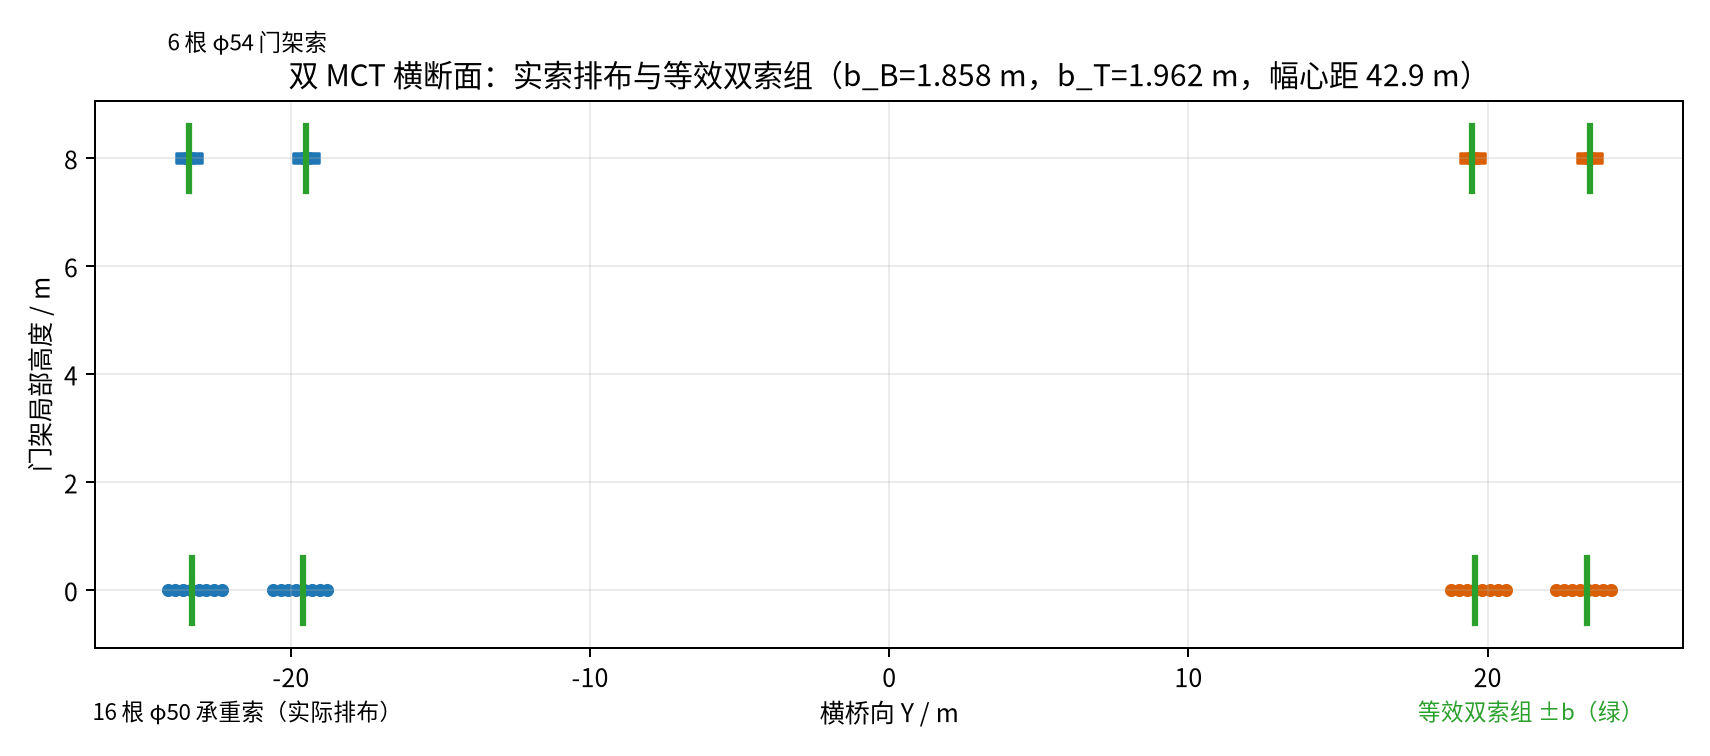
\includegraphics[width=0.94\linewidth]{../roll_upgraded_results/roll_upgraded_cross_section.png}
\caption{双 MCT 横断面：实索排布（点）与等效双索组位置（绿线）。}
\end{figure}

\section{推导一：双索组等效}\label{sec:twoline}

设一幅承重索束由 $n=16$ 根等份索组成，索 $i$ 位于横向偏距 $y_i$（对称排布），
单根张力 $T/n$、刚度 $EA/n$、线质量 $m/n$。把索束等效为位于 $\pm b$ 的两个索组
（各 $T/2$、$EA/2$、$m/2$），取
\begin{equation}\label{eq:rms}
b=\Big(\tfrac1n\textstyle\sum_i y_i^2\Big)^{1/2},
\qquad b_B=1.85809\ \text{m},\quad b_T=1.96152\ \text{m}.
\end{equation}

\textbf{命题 1（共模不变）}：两索组同相运动时，每组承担原索束一半的几何刚度
$\tfrac{T/2}{L}(\bm I-\bm n\bm n^{\mathsf T})$ 与弹性刚度 $\tfrac{EA/2}{L}\bm n\bm n^{\mathsf T}$，
合成后与原单索束方程逐项相同；质量同理。故 L/V/边跨各族动力学在拆分前后严格一致
（数值验证见表 \ref{tab:match}：升级后 LS1/VA1/LA1 等行仅因质量空间化移动 $\le0.5\%$）。

\textbf{命题 2（滚转二阶矩精确）}：幅内滚转场 $w_i(x)=y_i\,\theta(x)$ 的几何应变能与动能分别为
\begin{equation}
U=\tfrac12\textstyle\sum_i \tfrac{T}{n}\,y_i^2\!\int\!\theta'^2\,\mathrm dx
 =\tfrac12\,T b^2\!\int\!\theta'^2\,\mathrm dx,
\qquad
K=\tfrac12\, m b^2\!\int\!\dot\theta^2\,\mathrm dx ,
\end{equation}
在等张力分摊假设下（单根索承担束张力的 $1/n$），双索组模型把
$\sum_i T_i y_i^2$、$\sum_i (EA)_i y_i^2$、$\sum_i m_i y_i^2$ 全部精确保持。
对称竖弯/对称扭转分支的 Irvine 弹性附加张力项由 TENSTR 单元的 $EA$ 项自动携带，
无需另行推导。

\section{推导二：端口凝聚的滚转可观性与双簇端口}\label{sec:cluster}

\subsection{三种端口方案的运动学地位}

\textbf{(a) 单中心平动端口（旧正式 ROM）}：16 个索点刚性映射到一个中心
$\bm u_i=\bm u_c+\bm\theta_c\times\bm r_i$，再把 $\bm\theta_c$ 自由凝聚。平面模型只能观测
$\bm u_c$，滚转不可观：普通门架退化为秩一轴杆（5 个零机构），横通道 K12 在 T 族模态中
应变能 $\le0.34\%$。这是锁定诊断中扭转塌缩的直接原因。

\textbf{(b) 保留转角 + 刚性截面展开（本次首先尝试并否决）}：把保留 $\bm\theta_c$ 的
K12(6DOF)/K24 通过 $\bm u(\pm b)=\bm u_c\pm\bm\theta_c\times b\hat{\bm y}$ 的
Moore--Penrose 伪逆展开到双索组节点。展开在能量上与凝聚严格一致（映射零空间恰为审计
标定的不可观钻转 RY，属 $\bm K$ 的零模态），但它把整个 5.34 m 幅宽当成刚性平板：
Rayleigh 检验显示幅内滚转分支被推到 $1.5\text{--}3.8$ Hz（表 \ref{tab:rayleigh}），
比附件 TA1 高一个量级——\textbf{截面刚性是过约束}，横梁在索簇之间的挠曲柔性被非物理地锁死。

\textbf{(c) 双簇平动端口（本文方案）}：实索天然分两簇（承重索 $8+8$、门架索 $3+3$）。
把每簇刚性映射到该簇参考点（参考点取在 $\pm b$ 处——刚性映射对参考点选取不敏感，
取 rms 点使子端口与双索组节点\textbf{严格重合}），保留每簇 6 自由度后把全部转角自由凝聚：
\begin{equation}
\bm K_{\text{tt}}^{\text{cl}}=\bm K_{\text{tt}}-\bm K_{\text{tr}}\bm K_{\text{rr}}^{+}\bm K_{\text{tr}}^{\mathsf T},
\end{equation}
其中鞍点约束 $[\bm K\ \bm A^{\mathsf T};\ \bm A\ \bm 0]$ 施加索点—门架梁轴的 UXYZ 虚功一致映射
（与审计凝聚完全同一内核）。转角自由凝聚意味着\textbf{索不向门架传递弯矩}——这是物理事实，
不是简化。四/八个平动子端口张成的运动学已能客观表达截面滚转，且簇间横梁柔性保留。

\subsection{双簇凝聚的谱审计}

\begin{itemize}
  \item 门架（单品，4 子端口，12 平动）：恰 6 个刚体零模态 + 6 个正广义弹簧
        $\{90.6,\ 346.7,\ 2103.6,\ 1.73\times10^4,\ 1.44\times10^5,\ 4.76\times10^5\}$ N/mm，无机构；
  \item 横通道 + 两品门架（8 子端口，24 平动）：恰 6 个刚体零模态 + 18 个正弹簧
        （$1.61\text{--}2.47\times10^6$ N/mm），无机构；
  \item 轴向对照：簇端口门架轴向 $6262$ N/mm，低于单中心值 $24926$ N/mm——
        差值即截面刚性假设锁死的横梁挠曲柔性（表 4--1 各行门架轴向能量 $\sim10^{-6}$，
        对目标行无实质影响）；
  \item 刚体零空间在装配前逐矩阵校验（相对残差 $<10^{-6}$），随站位弦向/坡度旋转后严格保持。
\end{itemize}

与横通道 21 站的既有惯例一致，全部站位统一复用 H10 代表矩阵并旋转到站位弦向；
不再做每站轴向重标（该重标只对秩一轴杆定义良好）。

\section{推导三：二期质量的空间化分配}\label{sec:mass}

二期集中质量（963.811 t）原按平面 CONLOAD 全部落在幅中心线，滚转惯量为零。
本文改用质量空间化审计 V2.0 的逐点坐标 $(x_j,y_j,z_j,m_j)$：
纵向按链上相邻节点线性插值（保 $x$ 质心）；竖向取最近链层（承重/门架索层）；
横向在 $\pm b$ 双线间取保质心权重
\begin{equation}
w_{\pm}=\tfrac12\Big(1\pm\frac{\Delta y_j}{b}\Big),\qquad \Delta y_j=y_j-y_{\text{幅心}},
\end{equation}
幅间（$|y_j|<18$ m 的横通道构件，150.2 t）先按 $y$ 线性权重分配到两幅。
该分配精确保持总质量与横向一阶矩；二阶矩（滚转惯量）方面，逐幅二期质量的真实
rms 偏距为 2.077 m，双线表达为 $b_B=1.858$ m，对应侧向二期惯量低估约 20\%，
占全截面滚转惯量 1--2\%（索系质量占主导且精确）。总质量闭合
$4108.46690758$ t，误差 $9.7\times10^{-10}$ t，优于旧模型的 0.137 kg。

\section{实现与数值验证}\label{sec:impl}

升级模型：$2\times2\times1125=4500$ 节点、13500 平动自由度（自由 13284）；
80 阶广义特征值解（shift-invert）。验证链：
(i) APDL 源等价性：单中心 K24 复现差 0.0；
(ii) 簇矩阵谱与刚体零空间（上节）；
(iii) 特征对相对残差 $\le4.9\times10^{-10}$；最低频 0.0368 Hz，0.01 Hz 以下 0 阶；
(iv) 与锁定旧模型的前 24 阶质量加权 MAC 追踪（新向量按双线平均投影回中心线空间）：
主跨 L/V/T 行 MAC $0.94\text{--}0.99994$、频移 $\le1.1\%$，升级是受控细化而非模型漂移。

\section{结果}\label{sec:results}

\subsection{表 4--1 十四行正式配对（升级后 vs 锁定旧值）}

配对规则与锁定版同层级：主跨能量 $\ge0.65$ + 家族 + 奇偶性 + 家族内升频序号；
半波仅作指纹；边跨行按非主跨能量 + 全局一一指派。T 族信号升级为
"幅间差分竖向 + 幅内滚转"合并的系统扭转观测量（与锁定口径连续；
幅内纯滚转分支在本模型位于 1 Hz 以上、80 阶窗口之外）。

\begin{table}[h]\centering\small
\begin{tabular}{llrrrrrr}
\toprule
行 & 描述 & 附件 Hz & 旧配对 Hz & 旧误差 & 新配对 & 新 Hz & 新误差 \\
\midrule
LS1 & 一阶正对称横弯 & 0.0365 & 0.036773 & $+0.75\%$ & M1 & 0.036825 & $+0.89\%$ \\
VA1 & 一阶反对称竖弯 & 0.0700 & 0.071446 & $+2.07\%$ & M3 & 0.071142 & $+1.63\%$ \\
LA1 & 一阶反对称横弯 & 0.0726 & 0.073502 & $+1.24\%$ & M4 & 0.073147 & $+0.75\%$ \\
TA1 & 一阶反对称扭转 & 0.0996 & 0.071491 & $-28.22\%$ & M2 & 0.071093 & $\bm{-28.62\%}$ \\
VS1 & 一阶正对称竖弯 & 0.1028 & 0.101177 & $-1.58\%$ & M6 & 0.101626 & $-1.14\%$ \\
LS2 & 二阶正对称横弯 & 0.1087 & 0.110112 & $+1.30\%$ & M7 & 0.109799 & $+1.01\%$ \\
TS1 & 一阶正对称扭转 & 0.1147 & 0.100981 & $-11.96\%$ & M5 & 0.101135 & $\bm{-11.83\%}$ \\
SIDE1 & 边跨模态 & 0.1149 & 0.116182 & $+1.12\%$ & M8 & 0.120952 & $+5.27\%$ \\
SIDE2 & 边跨模态 & 0.1239 & 0.124815 & $+0.74\%$ & M9 & 0.125595 & $+1.37\%$ \\
VA2 & 二阶反对称竖弯 & 0.1438 & 0.146445 & $+1.84\%$ & M15 & 0.146060 & $+1.57\%$ \\
LA2 & 二阶反对称横弯 & 0.1449 & 0.146579 & $+1.16\%$ & M14 & 0.144864 & $-0.02\%$ \\
SIDE3 & 边跨模态 & 0.1557 & 0.164799 & $+5.84\%$ & M17 & 0.165908 & $+6.56\%$ \\
TS2 & 二阶正对称扭转 & 0.1571 & 0.143814 & $-8.46\%$ & M10 & 0.142913 & $\bm{-9.03\%}$ \\
VS2 & 二阶正对称竖弯 & 0.1744 & 0.145334 & $-16.67\%$ & M13 & 0.144424 & $-17.19\%$ \\
\midrule
\multicolumn{4}{l}{MAE / RMS（14 行）} & $5.92\%/9.78\%$ & & & $6.21\%/10.06\%$ \\
\multicolumn{4}{l}{T 族 / 非 T MAE} & $16.21\%/3.12\%$ & & & $16.49\%/3.40\%$ \\
\bottomrule
\end{tabular}
\caption{升级前后正式配对。主跨 L/V 行普遍改善（LA2 $+1.16\%\to-0.02\%$、
LA1 $+1.24\%\to+0.75\%$、VS1 $-1.58\%\to-1.14\%$、VA1 $+2.07\%\to+1.63\%$）；
\textbf{T 族三行几乎不动}；边跨行受二期质量空间化在短跨的 $x$ 向重分配影响变差
（SIDE1 $+1.12\%\to+5.27\%$），VS2 保持 $-17\%$ 量级不动。}
\label{tab:match}
\end{table}

\begin{figure}[h]\centering
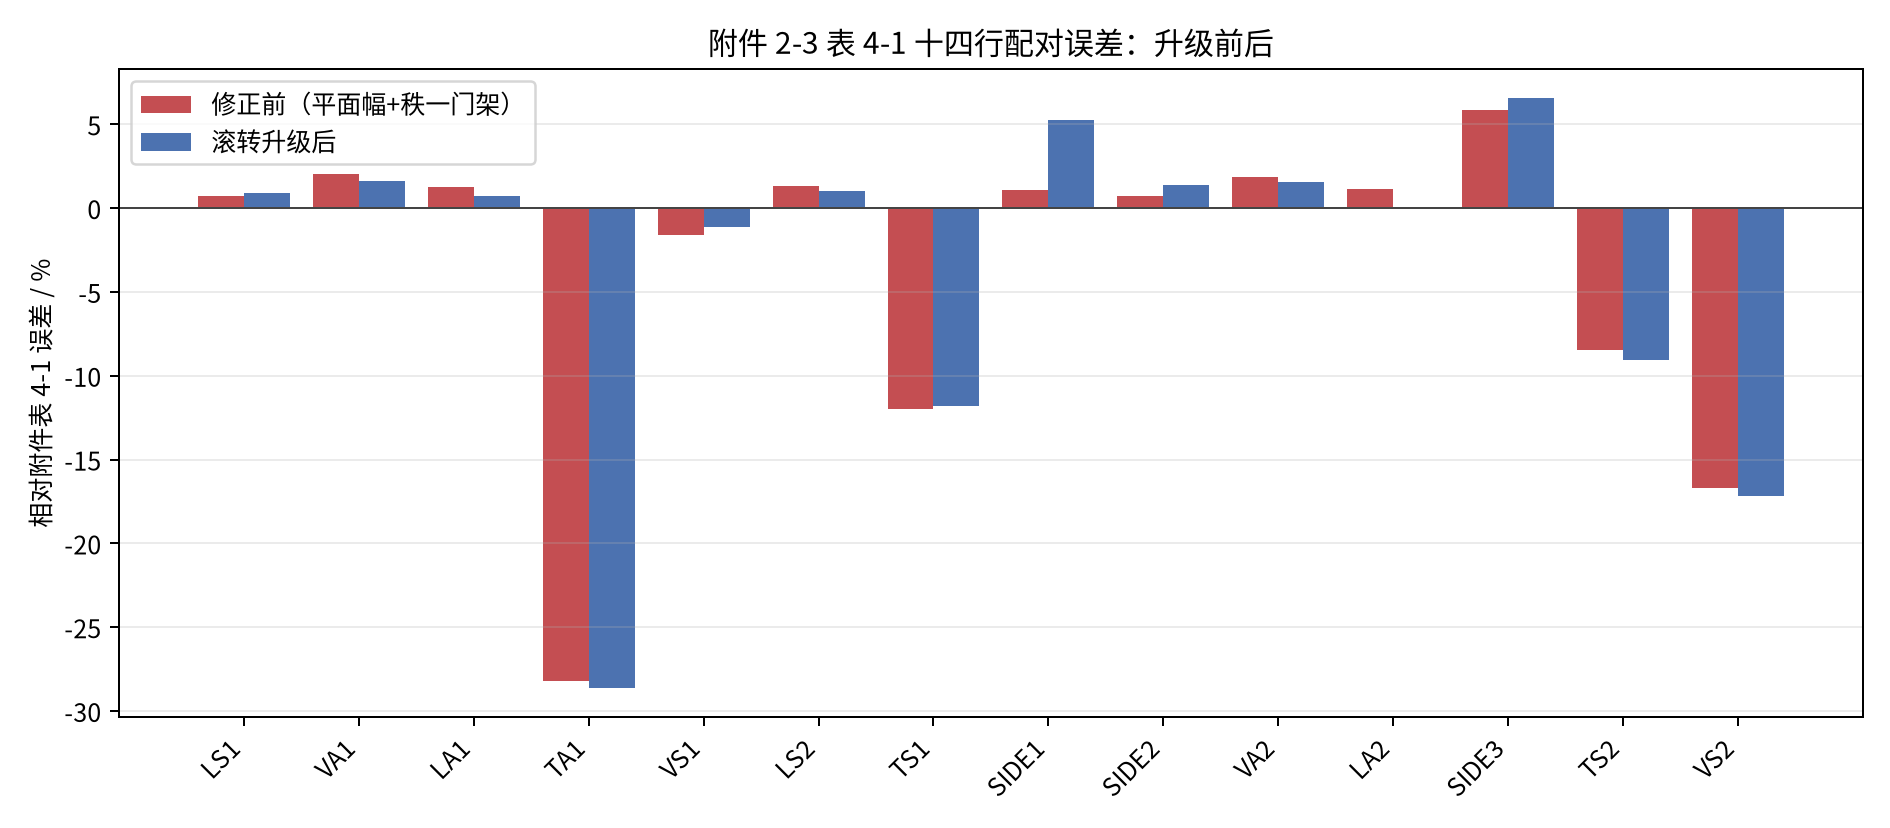
\includegraphics[width=0.98\linewidth]{../roll_upgraded_results/roll_upgraded_error_comparison.png}
\caption{十四行误差：升级前后对比。}
\end{figure}

\subsection{被治愈的非物理分支}

\begin{itemize}
  \item \textbf{双索组呼吸机构}：索组对开的"呼吸"模态在无簇端口时充斥 0.03--0.18 Hz
        （纯双线拆分的固有机构）；簇端口门架恢复横梁约束后全部消失；
  \item \textbf{门架索横向解耦分支}：旧模型自 M37（0.2804 Hz）起 13 阶门架索动能
        $>95\%$ 的敏感分支（秩一门架只能轴向握持门架索），升级后门架索被簇端口
        客观握持，该频段转化为受约束的系统横向分支（SYSY，0.26--0.32 Hz），
        原"局部 roll 不得升级为物理验收值"的限制自然解除。
\end{itemize}

\section{扭转可达域：为什么 T 族不动，以及附件隐含什么}\label{sec:reach}

\subsection{引理 A（系统扭转钉扎）}

双幅整体扭转（刚体旋转型模态 $w_i=\psi(x)\,y_i$）的频率比满足
\begin{equation}
\frac{\lambda_T}{\lambda_V}
=\frac{\sum_i T_i y_i^2\ \big/\ \sum_i m_i y_i^2}{\sum_i T_i\ \big/\ \sum_i m_i}.
\end{equation}
本结构张力与质量的横向分布同构（都集中在 $\pm21.45\pm b$ 的索线上，
幅间构件仅 150 t），故 $\lambda_T/\lambda_V\approx1$：\textbf{系统扭转被摆式物理
钉在竖弯族频率上}，与门架、横通道、索内力细节无关。数值证据：新模型
TA1--VA1 分裂 $0.069\%$，旧模型 $0.063\%$——两代完全不同的门架/横通道处理给出同一结果。
反对称系统扭转无净索伸长（Irvine 项为零），弹性也无法把它抬升。
要使 $\lambda_T/\lambda_V=1.423^2$，质量的横向 rms 必须缩到 15.1 m
（现约 21.5 m），即约一半质量移到幅间——与任何审计质量数据不符。

\subsection{引理 B（幅内滚转锁定）}

幅内滚转分支的位置由 Rayleigh 商在约束场族上标定：

\begin{table}[h]\centering\small
\begin{tabular}{lcccc}
\toprule
滚转场（$n=2$ 反对称） & 无侧摆 & 半侧摆 & 全侧摆（局部刚体） \\
\midrule
截面刚性展开方案 (b) & 3.82 Hz & 2.49 Hz & 1.51 Hz \\
双簇端口方案 (c)，双幅同相 & 3.64 Hz & 2.38 Hz & 1.46 Hz \\
双簇端口方案 (c)，双幅反相 & 2.76 Hz & 1.74 Hz & 1.05 Hz \\
\bottomrule
\end{tabular}
\caption{幅内滚转分支的 Rayleigh 频率（全侧摆=门架索层随刚体滚转侧移 $-h\theta$，
$h=8$ m）。附件 TA1 为 0.0996 Hz。}
\label{tab:rayleigh}
\end{table}

即使换成更柔的双簇端口，滚转分支仍在 $1.0$ Hz 以上。控制性刚度为审计钢结构的
滚转传递（对被索幕握持的接口做 Schur 凝聚）：
\begin{center}
\begin{tabular}{ll}
门架 B 簇对滚转（T 簇被握持） & $6.9\times10^{7}$ N·m/rad \\
门架 B/T 联合滚转（无侧摆） & $4.7\times10^{6}$ N·m/rad \\
横通道单侧接口刚体滚转（对幅固定） & $9.8\times10^{7}$ N·m/rad \\
横通道双幅同相滚转 & $2.6\times10^{8}$ N·m/rad \\
\end{tabular}
\end{center}

\subsection{附件隐含的滚转约束（反推）}

设幅内滚转仅由索幕摆式项 + 分布滚转弹簧 $k_\varphi$（N·m/rad/m）约束，则
\begin{equation}
k_\varphi=\big(\lambda_{\text{TA1}}^{\text{附件}}-\lambda_{\text{自由滚转}}\big)\,J_\ell,
\qquad
J_\ell=(m_B+m_{\text{二期}})\,b_B^2\approx1305\ \text{kg·m}^2/\text{m},
\end{equation}
代入 $\lambda^{附件}_{TA1}=(2\pi\times0.0996)^2$、$\lambda_{\text{自由}}=(2\pi\times0.0711)^2$：
$k_\varphi\approx251$ N·m/rad/m，按门架间距 59.6 m 折算\textbf{每品门架约
$1.5\times10^{4}$ N·m/rad}（按 TS1 反推为 $0.9\times10^{4}$，同量级）。
与审计值对比：比门架框架低 \textbf{2 个数量级}以上、比横通道刚接低 \textbf{4 个数量级}。

\textbf{结论}：附件表 4--1 的扭转频率\textbf{不可能}由现有审计部件（刚性 CERIG 连接的
门架/横通道钢结构 + 索幕）客观装配得到；它要求索—门架/横通道连接在滚转方向近似铰接
（夹具/滚轮式连接的量级）。修复所缺的不是装配方法，而是这一个连接柔度参数的设计出处。
在取得该参数前，任何把 T 族"调"到附件值的做法都等于把未知连接柔度当拟合旋钮，
不属于客观修复，本文不做。

\section{图纸连接构造与附件 2--3 原文核证（2026-08-27 补充）}\label{sec:drawings}

\subsection{图纸中的真实连接方式}

从 Release \texttt{zhangjinggao-full-20260729}（archive-0001）取得
《张靖皋长江大桥南航道桥猫道结构施工设计图》（1225 版，124 页；用户所指
《图纸汇总-2026.08.05.pdf》175 页为其后续汇总版，不在 2026-07-29 归档内）。
与扭转通路相关的连接构造（图证存于 \texttt{inputs/roll\_upgrade\_sources/drawing\_evidence/}）：

\begin{itemize}
  \item \textbf{承重索—门架}（MD1-04/05）：底梁 H175$\times$175$\times$7.5/11$\times$6150，
        16 个索位（两簇 $7\times260$）；每根 $\phi$50 承重索用一副 \textbf{M14 U 型螺栓}
        （JB/ZQ4321-2006，每套 32 只）抱夹于底梁——逐索点式传力，无弯矩约束，
        与凝聚采用的 UXYZ 运动学一致。
  \item \textbf{门架}（MD4-01/02）：$\Box$160$\times$160$\times$4 框架，顶梁 7380、
        立柱 5965、高 8000（可调 7.5--8.3 m，$\phi$16$\times$300 销 28 只）；
        顶部以楔块夹持 6-$\phi$54 门架承重绳。
  \item \textbf{横向通道}（MD5-03/04/09）：三角管桁架模块（9540 长、断面
        1500$\times$1700、弦 $\phi$152$\times$6）法兰拼接；图注"本标段共投入 12 道"
        （主跨 7、南边跨 3、南辅 2），与附件/模型的 21 站不同
        （"新增模块"图 MD5-07/08 提示后续增补，待 175 页汇总版核证）。
  \item \textbf{通道—猫道连接}（MD5-16/17、MD5-24/25）：通道支架经
        \textbf{MC 尼龙滚轮 $\phi$60$\times$50}（每套 32 只，间距 260 与索位一致）
        \textbf{骑在承重索上}；竖向支撑为 $\phi$34 销接管件加上下抱箍
        （R76 鞍座抱 $\phi$152 弦管，全桥 120 套，M16$\times$60）。
        \textbf{通道与门架之间不存在任何刚接节点}——审计 APDL 中把通道与门架
        焊死的 74 条 CERIG,ALL 刚臂是偏刚的理想化。
\end{itemize}

\subsection{图纸真实连接变体（drawing-soft）}

滚轮/销/抱箍连接传平动力而不传滚转矩——这恰是审计单中心平动 K12 的运动学内容
（滚转不可观、力耦合保留）。据此构造图纸柔性端变体：50 个普通站用双簇门架，
21 个通道站装配原审计 K12（经索组均值映射，滚转透明）。结果（\texttt{roll\_upgraded\_results\_drawing\_soft/}）：
非 T 族 MAE $3.39\%$，L/V 主跨行与刚接变体一致；
\textbf{T 族 $-28.66\%/-11.86\%/-9.15\%$}。
与刚接变体（$-28.62/-11.83/-9.03$）及锁定旧版（$-28.22/-11.96/-8.46$）对比：
\textbf{横跨"图纸柔性端—审计刚接端"的全部物理连接刚度区间，T 族误差漂移
$<0.7$ 个百分点}——引理 A 的钉扎结论被图纸证据反向加固。

\subsection{附件 2--3 原文核证}

从同一归档取得附件 2--3 原文（《张靖皋长江大桥南航道桥施工猫道抗风性能研究报告》，
西南交通大学风工程试验研究中心，32 页；SHA-256 \texttt{d17d4061\ldots} 与包 README
记录一致）。关键事实：

\begin{itemize}
  \item 表 4--1 出自报告自建 ANSYS 模型，其自述口径为："用索单元（link10）模拟猫道
        承重绳和门架承重绳，考虑索初始轴力对几何刚度的影响\ldots 用梁单元（beam4）
        模拟大小横梁、门架等等。因扶手立柱和扶手绳对猫道结构的整体刚度贡献甚小，
        因此只均布质量施加在猫道结构上。"
  \item \textbf{图 4-5（TA1 振型）的正视图为双幅反相竖向的 X 形交叉、侧视竖向近零}——
        与本文正式配对的系统扭转模态（M2/M8 族）为同一运动学形态；即附件的 TA1
        并非本文之外的某种未知形态，而是同一形态在其模型中算得 0.0996 Hz。
  \item 报告 §4.1 自述静风失稳由"横通道之间的小跨\ldots 跨中扭转角过大"控制，
        说明其模型中通道对扭转分跨起实质作用。
  \item V2 计算历程记录（2026-07-12/13）明确："现有资料没有提供 R19.2 源模型的完整
        ANSYS 输入\ldots 当前 V2 与附件源模型是否严格等价尚无完整证据"；且全部历史
        动力结果已于 2026-07-13 永久删除（"当前有效动力结果为 0 项"）——
        \textbf{迄今没有任何一个模型复现过表 4--1 的 T 行}。
\end{itemize}

\textbf{综合判定}：同一形态的系统扭转，其频率由引理 A 的分布比值钉定，与连接细节
无关；图纸柔性端与审计刚接端都不改变它。附件 TA1$=0.0996$ Hz 与其自述模型内容、
图纸连接构造和摆式物理三者联立后仍不可达。VS2（$-17\%$，对称高阶竖弯，对索系
弹性最敏感）的偏差模式指向索 EA/初张力状态口径差（如钢丝绳弹模取值差异即可产生
$+20\%$ 量级）。二者的最终定案都需要附件原始 ANSYS 输入（R19.2 源模型）——
这是"修复"链条上唯一缺失且必须外部索取的证据。

\begin{figure}[h]\centering
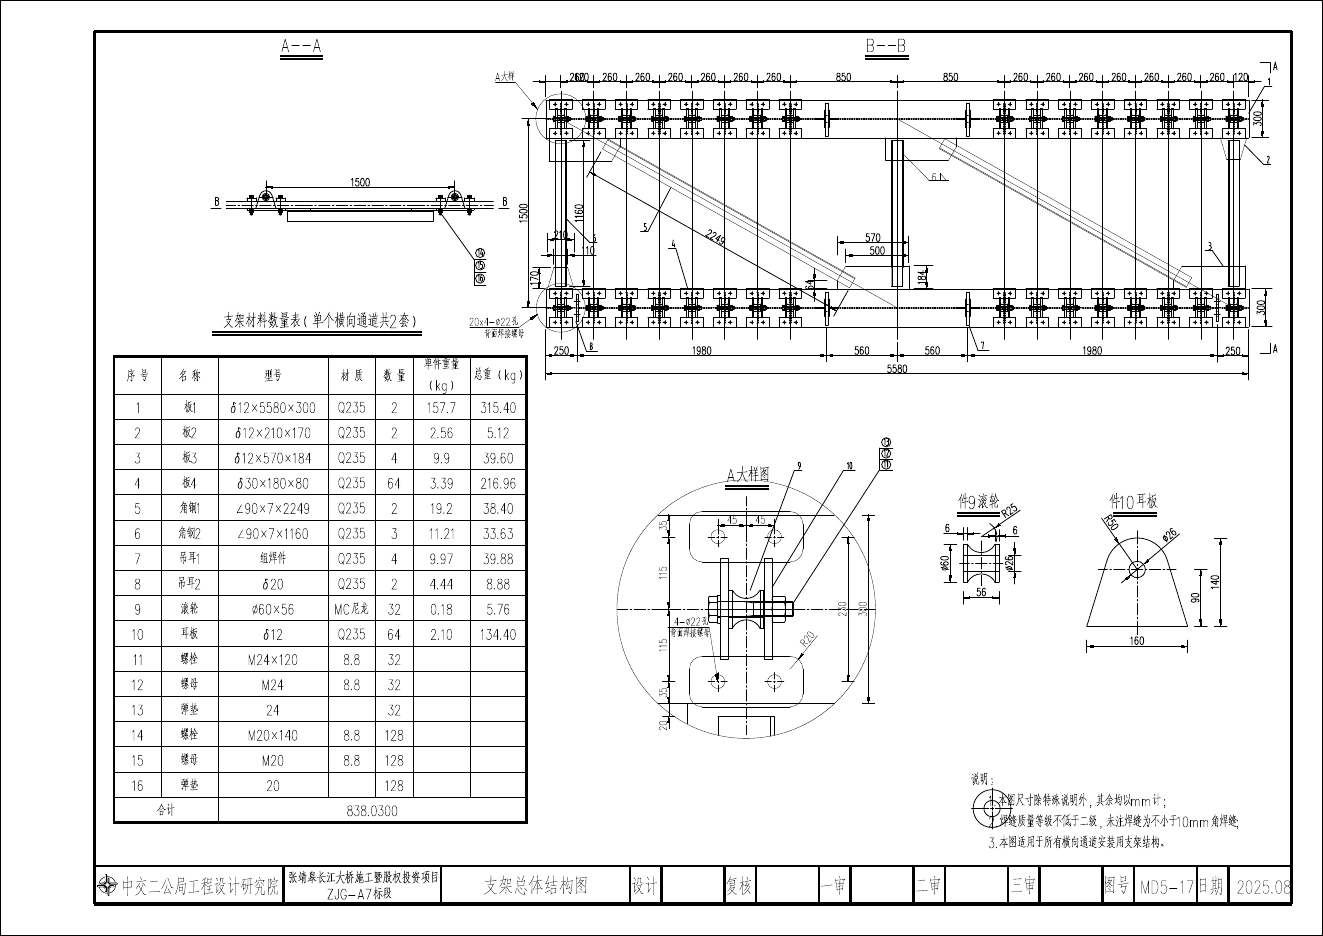
\includegraphics[width=0.48\linewidth]{../inputs/roll_upgrade_sources/drawing_evidence/MD5-17_support_nylon_rollers.png}
\hfill
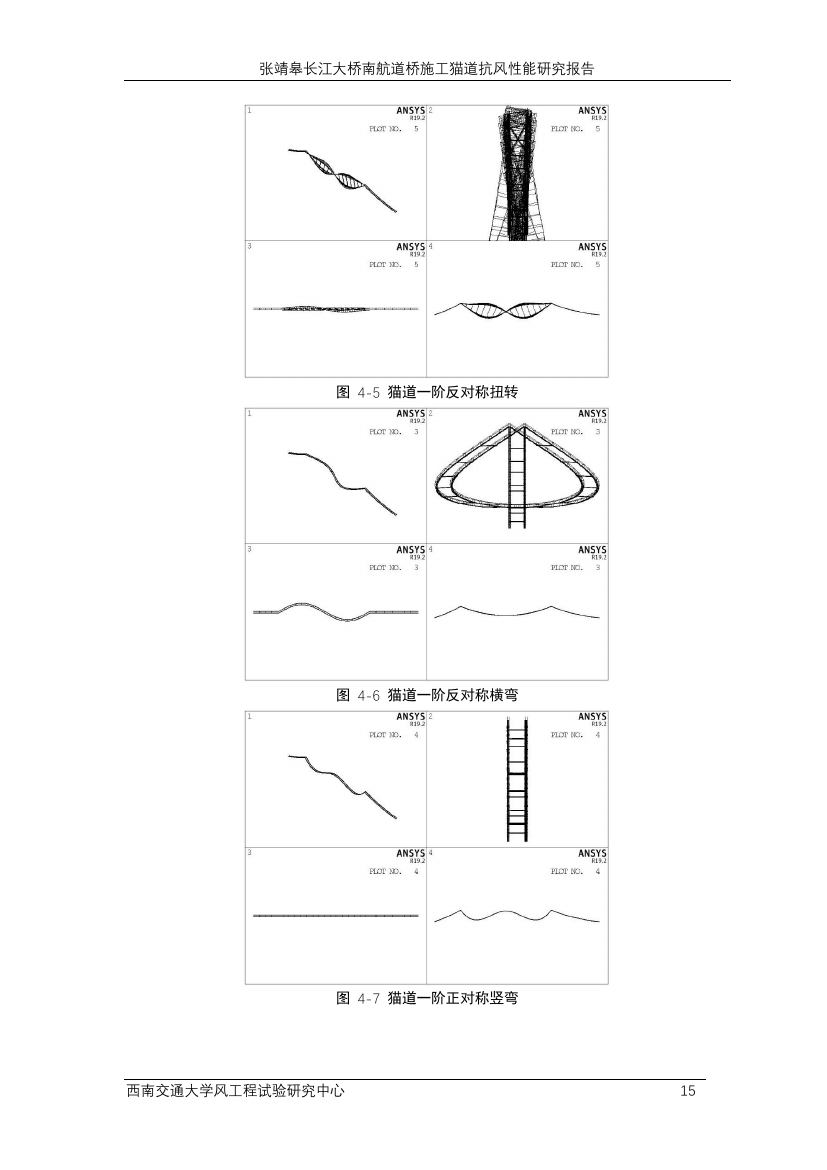
\includegraphics[width=0.48\linewidth]{../inputs/roll_upgrade_sources/drawing_evidence/attachment23_fig4-5_TA1_shape.png}
\caption{左：MD5-17 通道支架总体结构图（32 只 MC 尼龙滚轮 $\phi$60 骑在承重索上，
间距 260 与索位一致）。右：附件 2--3 图 4-5"猫道一阶反对称扭转"四视图——
正视图（右下）为双幅反相竖向 X 形交叉，与本文系统扭转模态同一形态。}
\end{figure}

\subsection{VS2 的独立性}

本次升级改变了门架、横通道、质量分布与滚转运动学的全部结构通路，VS2 仅从
$-16.67\%$ 移到 $-17.19\%$：其偏差与全部扭转/门架通路解耦，指向索系弹性状态
（张力/温度/弹模口径）或参考侧口径差异，维持"未定位"结论。

\section{能说什么 / 不能说什么}

\textbf{能说}：双索组 + 双簇端口 + 空间化质量的升级模型在结构层面修复了平面化
等效的全部三条缺失通路；主跨非扭转行改善或持平；两类非物理分支被治愈；系统扭转
钉扎与幅内滚转锁定两条引理把 T 族偏差从"未解释的模型误差"变为"审计部件的可达域
之外"的定量结论，并给出附件隐含连接柔度的数量级（$\sim10^4$ N·m/rad/品）。

\textbf{不能说}：不能宣布复现表 4--1（T 族 $-28.6/-11.8/-9.0\%$、VS2 $-17.2\%$、
边跨行 $+5\text{--}6.6\%$）；不能把反推的连接柔度当作设计事实使用（它是需求值，
不是来源值）；簇内刚性、H10 代表矩阵复用、等张力分摊、二期质量横向双线表达
均为显式近似；本文 not\_a\_scientific\_claim。

\appendix
\section{文件与复现}

代码：\texttt{code/condense\_h10\_cluster\_ports.py}（双簇凝聚）、
\texttt{code/double\_mct\_roll\_upgraded\_model.py}（升级模型 + 配对 + 追踪）。
数据：\texttt{inputs/roll\_upgrade\_sources/}（索耦合表、质量空间化表、APDL 源、
参考表、簇凝聚矩阵与审计 JSON）。结果：\texttt{roll\_upgraded\_results/}
（14 行配对、80 阶分类、新旧追踪、汇总 JSON 与图件）。复现：
\begin{verbatim}
python code/condense_h10_cluster_ports.py
python code/double_mct_roll_upgraded_model.py --modes 80
\end{verbatim}

\begin{figure}[h]\centering
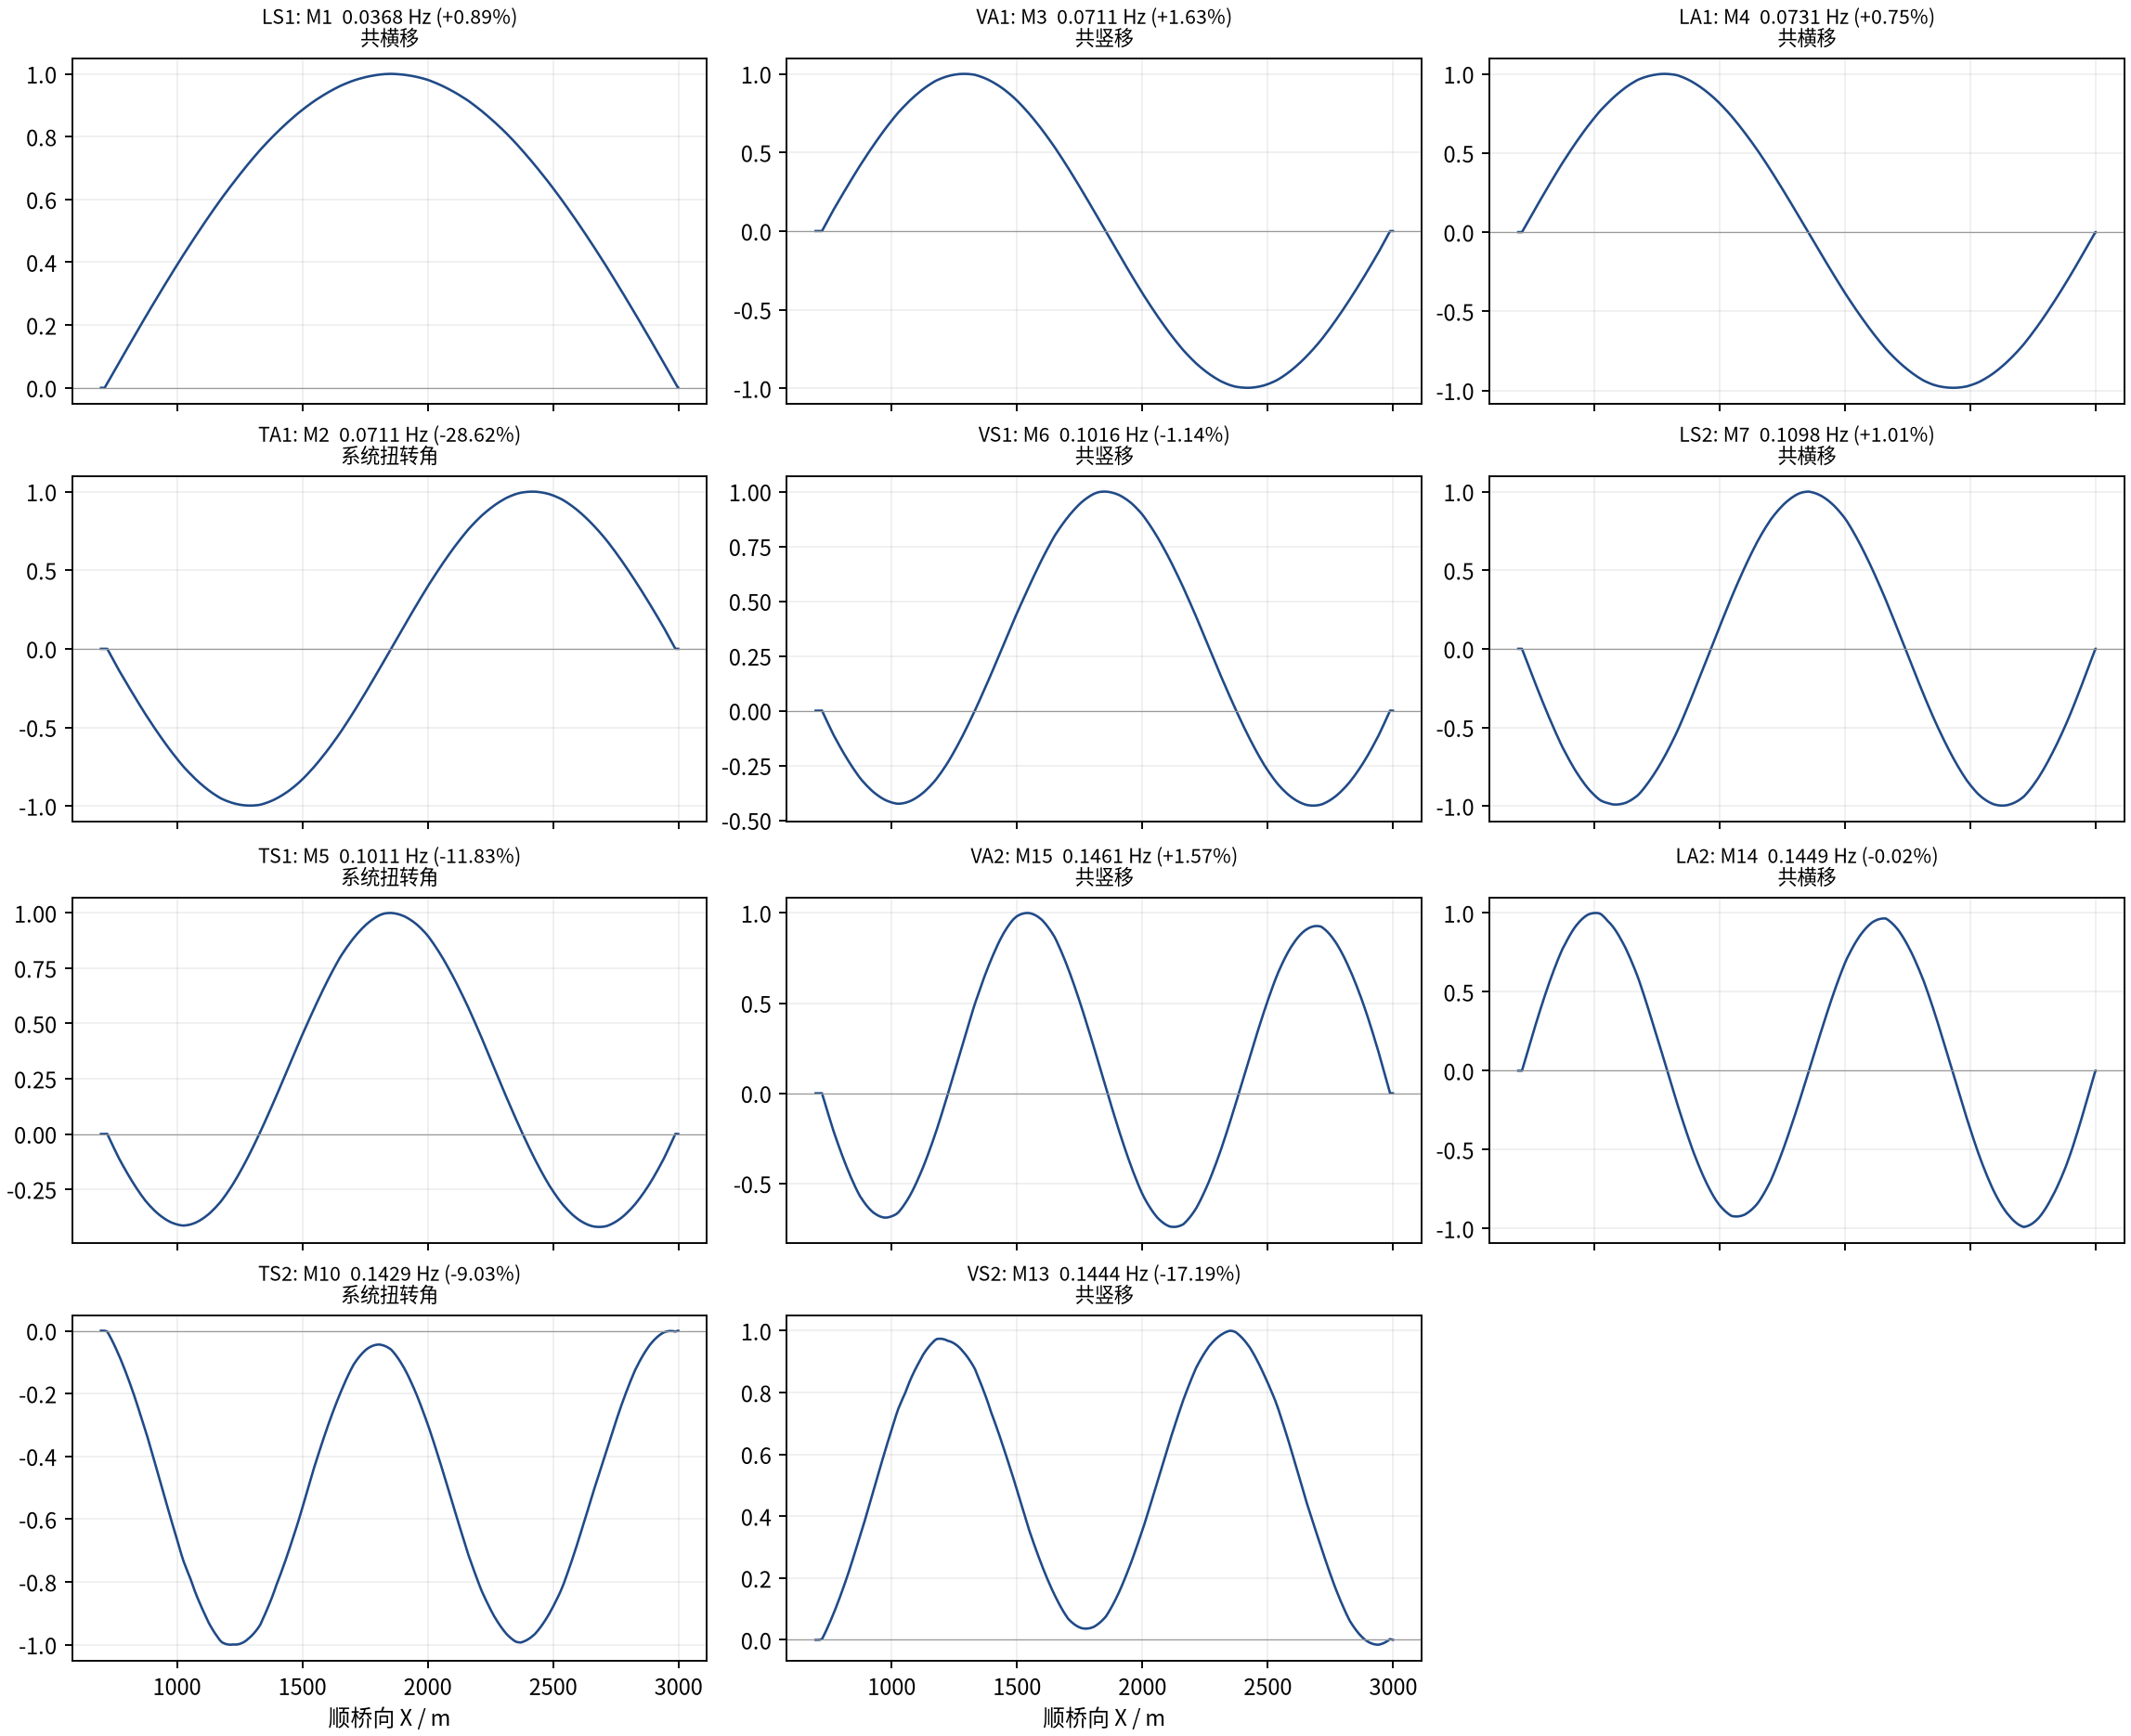
\includegraphics[width=0.99\linewidth]{../roll_upgraded_results/roll_upgraded_named_mode_shapes.png}
\caption{十一个具名行配对模态的主跨观测量形状（L：共横移；V：共竖移；T：系统扭转角）。}
\end{figure}

\end{document}
